\section{Introduction}
\label{sec:introduction-proplyd}

Proplyds are comet-like structures observed in HII regions like Orion Nebula Cluster (ONC). 
These objects are interpreted as a D-type Ionization Front (IF) of a photoevaporated flow 
originated in the protoplanetary disk of a nearby low mass YSO \citep{Johnstone:1998}.
The pressure of the surrounding gas is not enough to confine this flow \citep{HA:1998}
may be formed by the interaction of the photoevaporated wind of the proplyds with the stellar wind of \thC{}, which is highly supersonic $(M \sim 100)$. 

\begin{figure*}
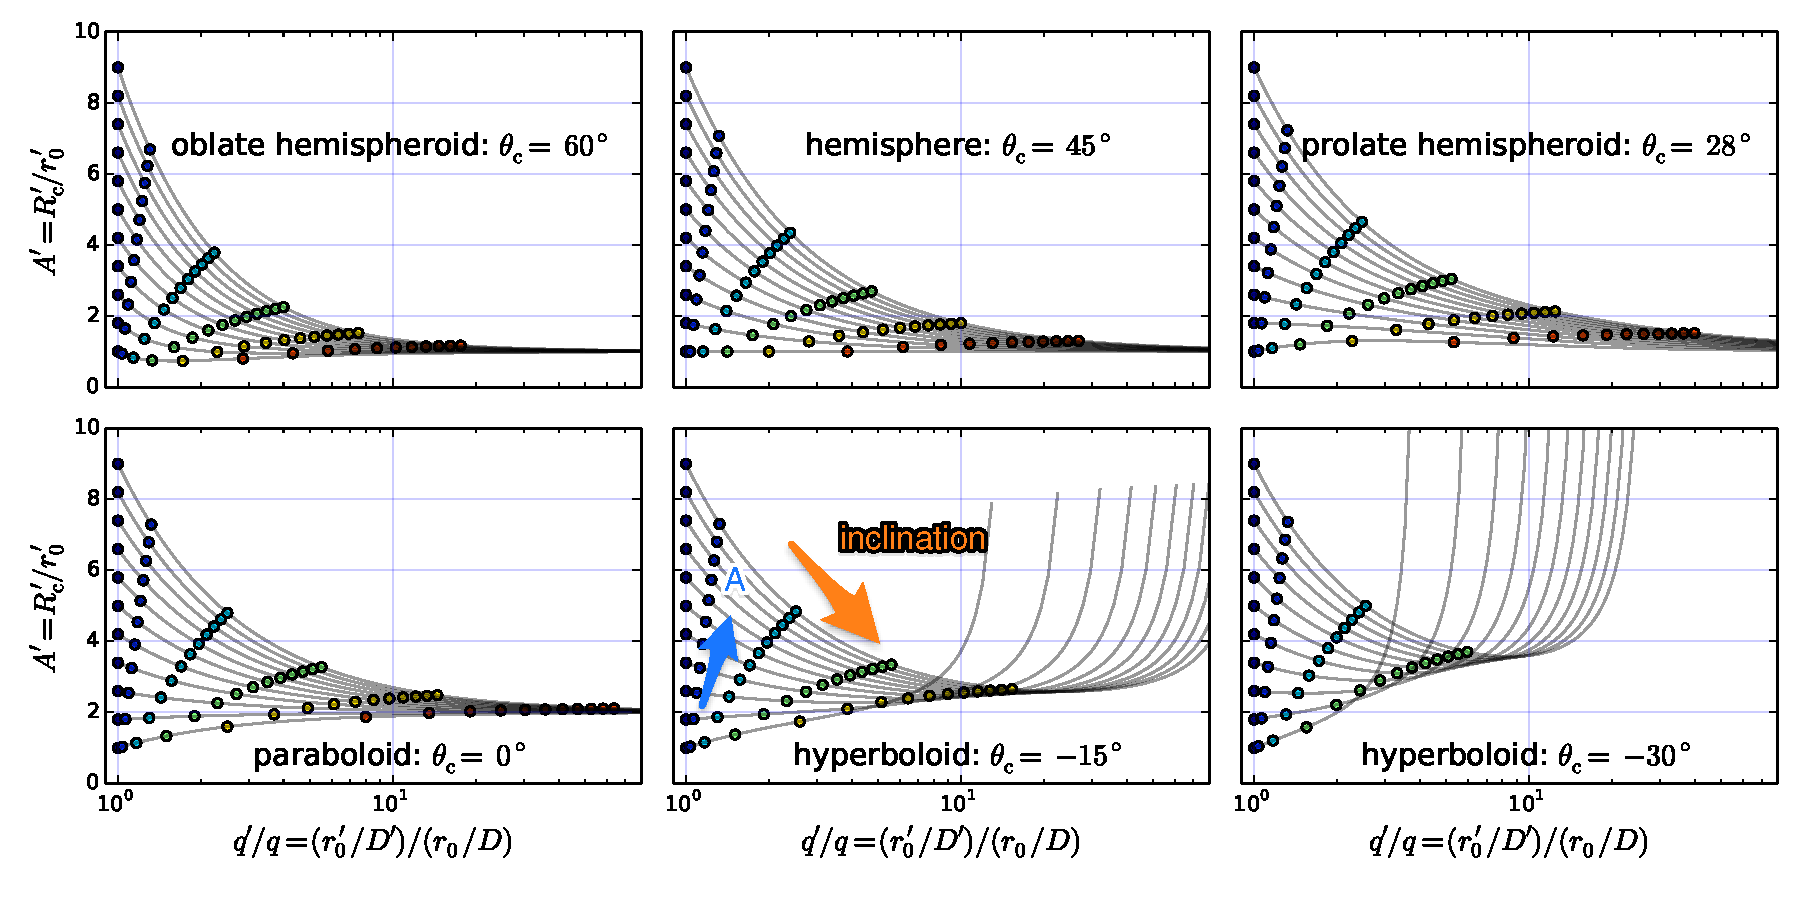
\includegraphics[width=0.9\linewidth]{annotated}
\caption{\textit{Moved here from the other paper, but we probably want
    to get rid of it completely at some point.} Projected Radius of
  curvature vs projected $R_0$ for
  $\theta_c=60^\circ,45^\circ,28^\circ, 0^\circ,-15^\circ,-30^\circ$. Each colored points represent
  the same shape at a different inclination. Being the dark blue the
  ones with the lower inclination and the red ones with the highest
  value. For closed shapes, there is an asymptotic limit for the
  projected radius of curvature at high inclinations, while for open
  shapes there is an upper limit for inclination where a tangent line
  can be observed.}
\label{fig:Apqp}
\end{figure*}

%%% Local Variables:
%%% mode: latex
%%% TeX-master: "proplyd-bowshocks"
%%% End:
